\documentclass[12pt,a4paper]{article}
\usepackage[english,romanian]{babel}
\usepackage[left=2.5cm,right = 2.5cm,top = 2.5cm, bottom = 2.5cm]{geometry}
\usepackage[utf8x]{inputenc}
\usepackage{graphicx}
\usepackage{listings}
\usepackage{enumerate}
\usepackage{hyperref}
\usepackage{amsmath}
\usepackage{ucs}
\usepackage[utf8x]{inputenc}
\lstset{breaklines=true}
\renewcommand{\baselinestretch}{1.5}

\begin{document}
\begin{titlepage}

\center

\textsc{ MINISTERUL EDUCAȚIEI REPUBLICII MOLDOVA}\\
\textbf{UNIVERSITATEA TEHNICĂ A MOLDOVEI}\\
\textbf{Facultatea "Calculatoare, informatică și microelectronică"}\\
\textsc{FILIERA ANGLOFONĂ}\\[2cm]

{ \huge \bfseries RAPORT}\\[0.5cm] % Title of your document
\textbf{Lucrarea de laborator nr. 3}\\
\textbf{TPI}\\[5cm]


\begin{minipage}{0.4\textwidth}
\begin{flushleft} \large
\emph{A efectuat:}\\
\end{flushleft}
\end{minipage}
~
\begin{minipage}{0.4\textwidth}
\begin{flushright} \large
Luca Victor\\
\end{flushright}
\end{minipage}\\[1cm]

\begin{minipage}{0.4\textwidth}
\begin{flushleft} \large
\emph{A verificat:}\\
\end{flushleft}
\end{minipage}
~
\begin{minipage}{0.4\textwidth}
\begin{flushright} \large
Zarea Ivan
\end{flushright}
\end{minipage}\\[4.5cm]

{\large Chișinău}\\
2014\\[3cm] % Date, change the \today to a set date if you want to be precise



\vfill % Fill the rest of the page with whitespace

\end{titlepage}
 \newpage

 \begin{center}
 \begin{Huge}
 \textbf{Laboratory work nr. 3}\\[0.2in]
 \end{Huge}
 \end{center}

\section*{Task 1}
 \subsection*{Frequency}

 What is the average total number of articles/day? How did that number grow
over time? Divide the data into two groups: Unimedia articles and Timpul
articles. Plot the growth of the number of articles for both sources. How does
that compare?

\subsection*{Program code}
Main part of the code:\\
\begin{lstlisting}
var averageNumberOfArticlesPerDay = function(articles) {
  var last  = moment(_.last(articles).datetime);
  var first = moment(_.first(articles).datetime);
  var nr_days  = last.diff(first, 'days');

  return articles.length / nr_days;
}

var sorted_articles  = sortArticles(articles);

  var counted_articles_per_month = _.countBy(sorted_articles, function(article) {
    year  = article.datetime.year();
    month = article.datetime.month();
    var newdate = moment().year(year).month(month).date(0).hours(0).minutes(0).seconds(0);
    return newdate.toDate();
  });

  var array_articles = [];
  counted_articles_per_month = _.pairs(counted_articles_per_month);
  _.each(counted_articles_per_month, function(article) {
    array_articles.push({
      "date":   moment(article[0]).toDate(),
      "value":  article[1]
    });
  });

  var unimedia = _.where(sorted_articles, {source : "unimedia"});
  var timpul   = _.where(sorted_articles, {source : "timpul"});

  var counted_articles_per_month_unimedia = _.countBy(unimedia, function(article) {
    year  = article.datetime.year();
    month = article.datetime.month();
    var newdate_unimedia = moment().year(year).month(month).date(0).hours(0).minutes(0).seconds(0);
    return newdate_unimedia.toDate();
  });

  var counted_articles_per_month_timpul = _.countBy(timpul, function(article) {
    year  = article.datetime.year();
    month = article.datetime.month();
    var newdate_timpul = moment().year(year).month(month).date(0).hours(0).minutes(0).seconds(0);
    return newdate_timpul.toDate();
  });

  var array_articles_unimedia = [];
  counted_articles_per_month_unimedia = _.pairs(counted_articles_per_month_unimedia);
  _.each(counted_articles_per_month_unimedia, function(article) {
    array_articles_unimedia.push({"date" : moment(article[0]).toDate(), "value1" : article[1]});
  });

  var array_articles_timpul = [];
  counted_articles_per_month_timpul = _.pairs(counted_articles_per_month_timpul);
  _.each(counted_articles_per_month_timpul, function(article) {
    array_articles_timpul.push({"date" : moment(article[0]).toDate(), "value2" : article[1]});
  });

\end{lstlisting}

\subsection*{Line chart}
\begin{center}
 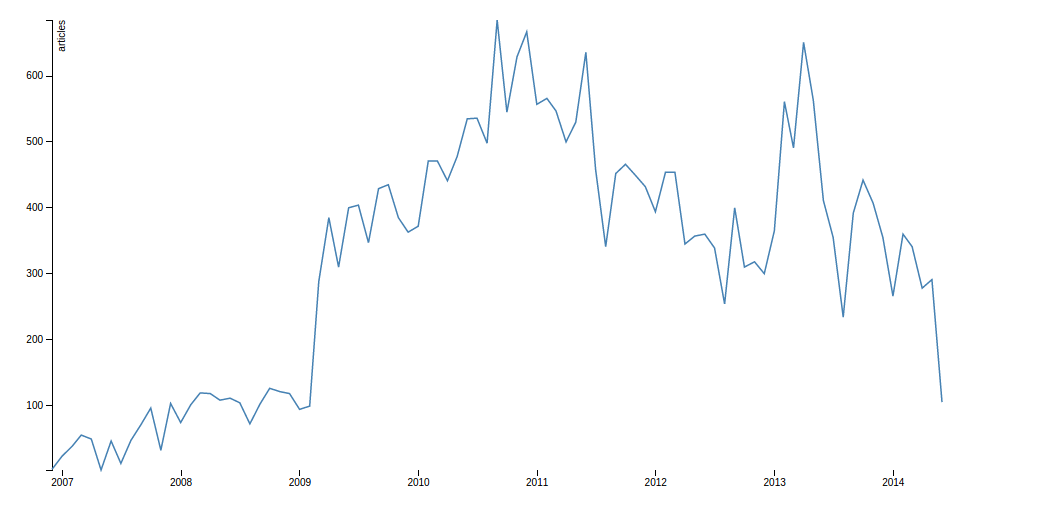
\includegraphics[width=6in]{Lab3d1.png}
 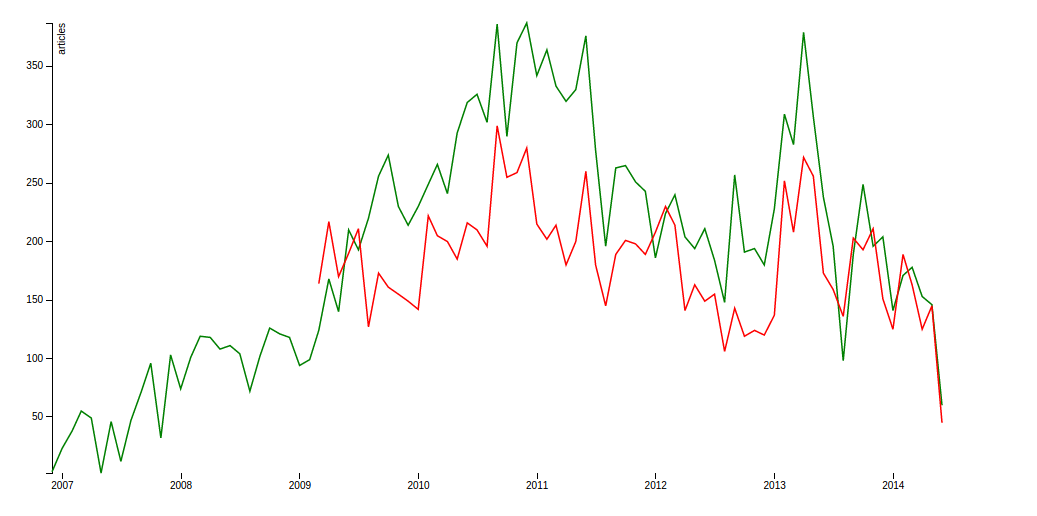
\includegraphics[width=6in]{Lab3d2.png}
\end{center}

\subsection*{Result}
Average total number of articles per day is 10.65.


\section*{Task 3}
 \subsection*{Views}
 For Unimedia, what is the average number of view/article/month? How did
that number evolve over time?

\subsection*{Program code}
\begin{lstlisting}
  var new_array = _.map(articles, function(article) {
    return {
      views:  article.views,
      date:   article.datetime
    }
  });

  var grouped_by_month = _.groupBy(new_array, function(article) {
    year  = article.date.year();
    month = article.date.month();
    var newdate_timpul = moment().year(year).month(month + 1).date(0).hours(0).minutes(0).seconds(0);
    return newdate_timpul.toDate();
  });


  grouped_by_month = _.pairs(grouped_by_month);

  _.each(grouped_by_month, function(property) {
    property[0] = moment(property[0]).toDate();
  });

  var sorted_by_month = _.sortBy(grouped_by_month, function(property) {
    return property[0];
  });

  var average_views_per_month_array = [];
  _.each(sorted_by_month, function(property) {
    var average_views_per_month = 0;
    average_views_per_month = _.reduce(property[1], function(memo, article) {
      return memo + article.views;
    }, 0);

    average_views_per_month_array.push({
      "date":   property[0],
      "value3": average_views_per_month / property[1].length
    });
  });
\end{lstlisting}

\subsection*{Line chart}
\begin{center}
 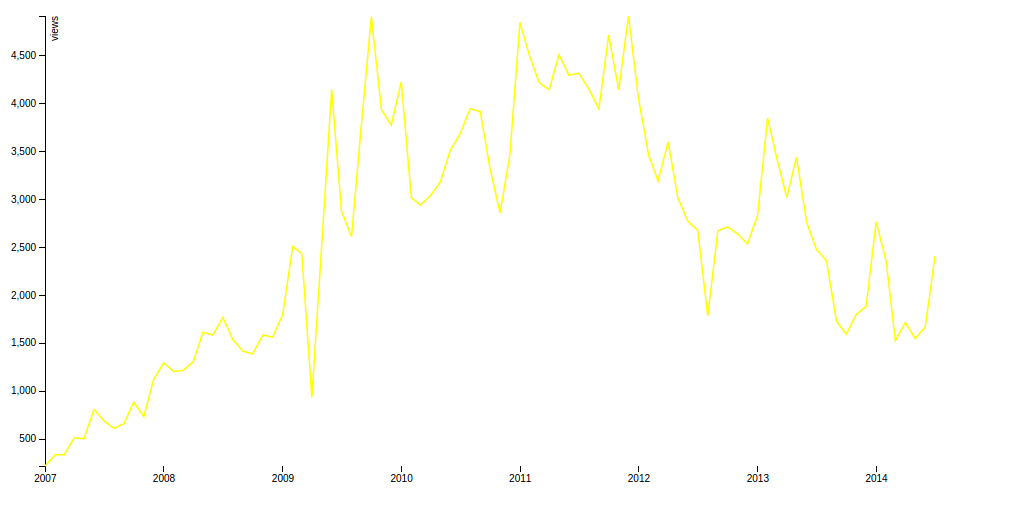
\includegraphics[width=6in]{Lab3d3.png}
\end{center}


\section*{Task 4}

\subsection*{Engineering linkbait}
Select articles that have (video) in their titles and ones that don’t. Create a
histogram of both of them. Do you see any statistically significant difference?\\
Plot the two curves: the growth of the number of views for all articles and
the growth of the number of views for articles that have (video). Do you see
anything?
\subsection*{Program code}
\begin{lstlisting}
Main part of the code:

var articles_with_video = _.filter(articles, function(article) {
  return article.title.indexOf("video")  >= 0 || article.title.indexOf("Video")  >= 0 ||
    article.title.indexOf("VIDEO")  >= 0;
 });

var articles_without_video = _.filter(articles, function(article) {
  return article.title.indexOf("video")  == -1 && article.title.indexOf("Video")  == -1 &&
    article.title.indexOf("VIDEO")  == -1;
  });

\end{lstlisting}

\subsection*{Histogram}
\begin{center}
  
\includegraphics[width=6in]{Lab3d5.png}
\end{center}
\begin{center}
\subsection*{Line chart}
  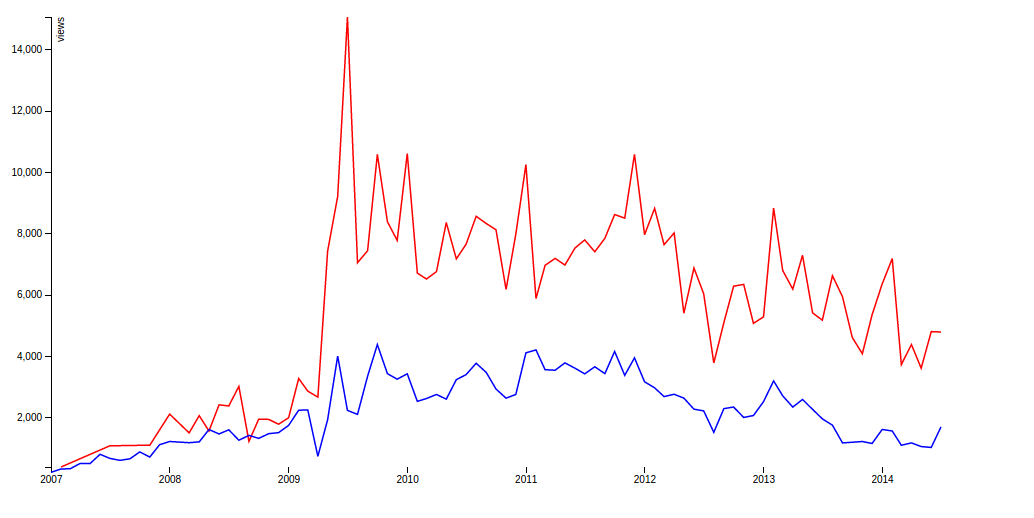
\includegraphics[width=6in]{Lab3d4.png}
  \end{center}


\section*{Task 5}

\subsection*{Conditional}
What is the probability that an article will have more than average views given
that it has the word ”VIDEO” in it?

\subsection*{Program code}
\begin{lstlisting}
//average of views for articles
  var nr_of_views = _.reduce(articles, function(memo, article) {
      return memo + article.views;
    }, 0);
  var average_nr_of_views = nr_of_views / articles.length;
  //average of views for articles with video
  var nr_of_views_for_articles_with_video = _.reduce(articles_with_video, function(memo, article) {
      return memo + article.views;
    }, 0);
  var average_nr_of_views_for_articles_with_video = nr_of_views_for_articles_with_video / articles_with_video.length;
  var articles_that_have_more_average_views = [];
  articles_that_have_more_average_views = _.filter(articles_with_video, function(article) {
    return article.views > average_nr_of_views;
  });
  var Probability = articles_that_have_more_average_views.length / articles_with_video.length * 100;
  console.log("Probability is: " + Probability + "%");

\end{lstlisting}
\subsection*{Result}
Probability that an article will have more than average views given
that it has the word ”VIDEO” in it: 76.7980820458178 \%

\subsection*{Conclusion:}

Playing with data becomes a lot more easier if we use additional libraries. In this laboratory work I used underscore, moment and
d3. On the first view this laboratory work seemed to be clear and easy, but after a couple of days spent in front of the screen I finally understood that it's not as easy as it seemed. An important step was to parse date from json in order to use moment date object for computing our tasks. Also it's important to mention that in order to build charts in d3 it is necessary to transform input data for d3 into an array of objects with two propreties: date and value.\\
  \par Results obtained in histogram show that nr. of articles which contain word "VIDEO" is much smaller than those how don't. An intersting fact we can notice is that average nr of views is definitely higher for the articles which contain "VIDEO".


\end{document}